\documentclass{article}
\usepackage[utf8]{inputenc}
\usepackage{graphicx}
\usepackage{geometry}
\usepackage{amsmath}
\usepackage{amsfonts}
\usepackage{float}
\usepackage{caption}
\usepackage{subcaption}
\usepackage{enumitem}

\geometry{left=25mm, top=25mm, right=25mm, bottom=25mm}

\title{PHY407 Lab 8}
\author{Pierino Zindel (1002429703) and Hayden Johnson (1002103537)}
\date{November 2, 2018}

\begin{document}

\maketitle

\noindent \textbf{Distribution of work:} Question 1 was completed by Pierino. Question 2 was completed by Hayden.

\section{Temperature Distribution in a Heat Conductor}

\subsection{Part b)}

We seek to evaluate the impact of overrelaxation by examining the solution to the heat equation with the given boundary conditions after 100 iterations using both regular relaxation ($w=0$) and overrelaxation with $w=0.9$. 

\begin{figure}[H]
	\centering
	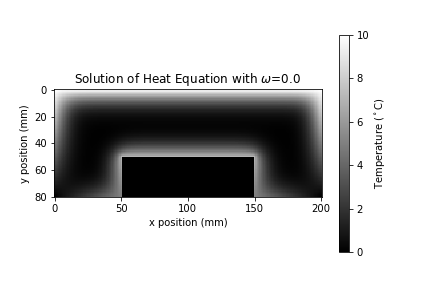
\includegraphics[width=0.8\textwidth]{../images/q1_b_0p0.png}
	\caption{Plot of temperature distribution after 100 iterations using Gauss-Seidel method, with regular relaxation ($w=0.0$).}
	\label{fig:1b_w=0.0}
\end{figure}

\begin{figure}[H]
	\centering
	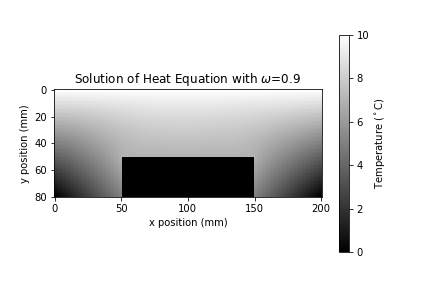
\includegraphics[width=0.8\textwidth]{../images/q1_b_0p9.png}
	\caption{Plot of temperature distribution after 100 iterations using Gauss-Seidel method, with overrelaxation ($w=0.9$).}
	\label{fig:1b_w=0.9}
\end{figure}

\subsection{Part c)}

\begin{figure}[H]
	\centering
	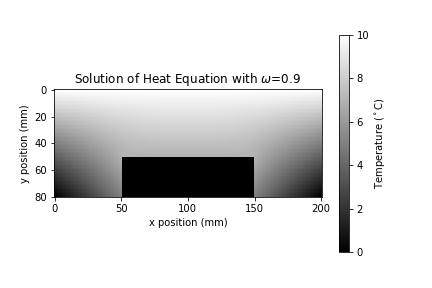
\includegraphics[width=0.8\textwidth]{../images/q1_c.png}
	\caption{Plot of temperature distribution created using Gauss-Seidel method, with overrelaxation ($w=0.9$), with a target precision of $1.0\times 10^{-6}$.}
	\label{fig:1b_w=0.9}
\end{figure}


\end{document}